
%\documentclass[11pts,a4paper,amsmath,amssymb,floatfix]{article}%{report}%{book}
\documentclass[12pts,a4paper,amsmath,amssymb,floatfix]{article}%{report}%{book}
\usepackage{graphicx,wrapfig,pdfpages}% Include figure files
%\usepackage{dcolumn,enumerate}% Align table columns on decimal point
\usepackage{enumerate,enumitem}% Align table columns on decimal point
\usepackage{bm,dpfloat}% bold math
\usepackage[pdftex,bookmarks,colorlinks=true,urlcolor=rltblue,citecolor=blue]{hyperref}
\usepackage{amsfonts,amsmath,amssymb,stmaryrd,indentfirst}
\usepackage{times,psfrag}
\usepackage{natbib}
\usepackage{color}
\usepackage{units}
\usepackage{rotating}
\usepackage{multirow}


\usepackage{pifont}
\usepackage{subfigure}
\usepackage{subeqnarray}
\usepackage{ifthen}

\usepackage{supertabular}
\usepackage{moreverb}
\usepackage{listings}
\usepackage{palatino}
%\usepackage{doi}
\usepackage{longtable}
\usepackage{float}
\usepackage{perpage}
\MakeSorted{figure}
%\usepackage{pdflscape}


%\usepackage{booktabs}
%\newcommand{\ra}[1]{\renewcommand{\arraystretch}{#1}}


\definecolor{rltblue}{rgb}{0,0,0.75}


%\usepackage{natbib}
\usepackage{fancyhdr} %%%%
\pagestyle{fancy}%%%%
% with this we ensure that the chapter and section
% headings are in lowercase
%%%%\renewcommand{\chaptermark}[1]{\markboth{#1}{}}
\renewcommand{\sectionmark}[1]{\markright{\thesection\ #1}}
\fancyhf{} %delete the current section for header and footer
\fancyhead[LE,RO]{\bfseries\thepage}
\fancyhead[LO]{\bfseries\rightmark}
\fancyhead[RE]{\bfseries\leftmark}
\renewcommand{\headrulewidth}{0.5pt}
% make space for the rule
\fancypagestyle{plain}{%
\fancyhead{} %get rid of the headers on plain pages
\renewcommand{\headrulewidth}{0pt} % and the line
}

\def\newblock{\hskip .11em plus .33em minus .07em}
\usepackage{color}

%\usepackage{makeidx}
%\makeindex

\setlength\textwidth      {16.cm}
\setlength\textheight     {22.6cm}
\setlength\oddsidemargin  {-0.3cm}
\setlength\evensidemargin {0.3cm}

\setlength\headheight{14.49998pt} 
\setlength\topmargin{0.0cm}
\setlength\headsep{1.cm}
\setlength\footskip{1.cm}
\setlength\parskip{0pt}
\setlength\parindent{0pt}


%%%
%%% Headers and Footers
\lhead[] {\text{\small{EX3029 -- Chemical Thermodynamics}}} 
\rhead[] {{\text{\small{Tutorial 02}}}}
%\chead[] {\text{\small{Session 2012/13}}} 
\lfoot[]{Dr Jeff Gomes}
%\cfoot[\thepage]{\thepage}
\rfoot[\text{\small{\thepage}}]{\thepage}
\renewcommand{\headrulewidth}{0.8pt}


%%%
%%% space between lines
%%%
\renewcommand{\baselinestretch}{1.5}

\newenvironment{VarDescription}[1]%
  {\begin{list}{}{\renewcommand{\makelabel}[1]{\textbf{##1:}\hfil}%
    \settowidth{\labelwidth}{\textbf{#1:}}%
    \setlength{\leftmargin}{\labelwidth}\addtolength{\leftmargin}{\labelsep}}}%
  {\end{list}}

%%%%%%%%%%%%%%%%%%%%%%%%%%%%%%%%%%%%%%%%%%%
%%%%%%                              %%%%%%%
%%%%%%      NOTATION SECTION        %%%%%%%
%%%%%%                              %%%%%%%
%%%%%%%%%%%%%%%%%%%%%%%%%%%%%%%%%%%%%%%%%%%

% Text abbreviations.
\newcommand{\ie}{{\em{i.e., }}}
\newcommand{\eg}{{\em{e.g., }}}
\newcommand{\cf}{{\em{cf., }}}
\newcommand{\wrt}{with respect to}
\newcommand{\lhs}{left hand side}
\newcommand{\rhs}{right hand side}
% Commands definining mathematical notation.

% This is for quantities which are physically vectors.
\renewcommand{\vec}[1]{{\mbox{\boldmath$#1$}}}
% Physical rank 2 tensors
\newcommand{\tensor}[1]{\overline{\overline{#1}}}
% This is for vectors formed of the value of a quantity at each node.
\newcommand{\dvec}[1]{\underline{#1}}
% This is for matrices in the discrete system.
\newcommand{\mat}[1]{\mathrm{#1}}


\DeclareMathOperator{\sgn}{sgn}
\newtheorem{thm}{Theorem}[section]
\newtheorem{lemma}[thm]{Lemma}

%\newcommand\qed{\hfill\mbox{$\Box$}}
\newcommand{\re}{{\mathrm{I}\hspace{-0.2em}\mathrm{R}}}
\newcommand{\inner}[2]{\langle#1,#2\rangle}
\renewcommand\leq{\leqslant}
\renewcommand\geq{\geqslant}
\renewcommand\le{\leqslant}
\renewcommand\ge{\geqslant}
\renewcommand\epsilon{\varepsilon}
\newcommand\eps{\varepsilon}
\renewcommand\phi{\varphi}
\newcommand{\bmF}{\vec{F}}
\newcommand{\bmphi}{\vec{\phi}}
\newcommand{\bmn}{\vec{n}}
\newcommand{\bmns}{{\textrm{\scriptsize{\boldmath $n$}}}}
\newcommand{\bmi}{\vec{i}}
\newcommand{\bmj}{\vec{j}}
\newcommand{\bmk}{\vec{k}}
\newcommand{\bmx}{\vec{x}}
\newcommand{\bmu}{\vec{u}}
\newcommand{\bmv}{\vec{v}}
\newcommand{\bmr}{\vec{r}}
\newcommand{\bma}{\vec{a}}
\newcommand{\bmg}{\vec{g}}
\newcommand{\bmU}{\vec{U}}
\newcommand{\bmI}{\vec{I}}
\newcommand{\bmq}{\vec{q}}
\newcommand{\bmT}{\vec{T}}
\newcommand{\bmM}{\vec{M}}
\newcommand{\bmtau}{\vec{\tau}}
\newcommand{\bmOmega}{\vec{\Omega}}
\newcommand{\pp}{\partial}
\newcommand{\kaptens}{\tensor{\kappa}}
\newcommand{\tautens}{\tensor{\tau}}
\newcommand{\sigtens}{\tensor{\sigma}}
\newcommand{\etens}{\tensor{\dot\epsilon}}
\newcommand{\ktens}{\tensor{k}}
\newcommand{\half}{{\textstyle \frac{1}{2}}}
\newcommand{\tote}{E}
\newcommand{\inte}{e}
\newcommand{\strt}{\dot\epsilon}
\newcommand{\modu}{|\bmu|}
% Derivatives
\renewcommand{\d}{\mathrm{d}}
\newcommand{\D}{\mathrm{D}}
\newcommand{\ddx}[2][x]{\frac{\d#2}{\d#1}}
\newcommand{\ddxx}[2][x]{\frac{\d^2#2}{\d#1^2}}
\newcommand{\ddt}[2][t]{\frac{\d#2}{\d#1}}
\newcommand{\ddtt}[2][t]{\frac{\d^2#2}{\d#1^2}}
\newcommand{\ppx}[2][x]{\frac{\partial#2}{\partial#1}}
\newcommand{\ppxx}[2][x]{\frac{\partial^2#2}{\partial#1^2}}
\newcommand{\ppt}[2][t]{\frac{\partial#2}{\partial#1}}
\newcommand{\pptt}[2][t]{\frac{\partial^2#2}{\partial#1^2}}
\newcommand{\DDx}[2][x]{\frac{\D#2}{\D#1}}
\newcommand{\DDxx}[2][x]{\frac{\D^2#2}{\D#1^2}}
\newcommand{\DDt}[2][t]{\frac{\D#2}{\D#1}}
\newcommand{\DDtt}[2][t]{\frac{\D^2#2}{\D#1^2}}
% Norms
\newcommand{\Ltwo}{\ensuremath{L_2} }
% Basis functions
\newcommand{\Qone}{\ensuremath{Q_1} }
\newcommand{\Qtwo}{\ensuremath{Q_2} }
\newcommand{\Qthree}{\ensuremath{Q_3} }
\newcommand{\QN}{\ensuremath{Q_N} }
\newcommand{\Pzero}{\ensuremath{P_0} }
\newcommand{\Pone}{\ensuremath{P_1} }
\newcommand{\Ptwo}{\ensuremath{P_2} }
\newcommand{\Pthree}{\ensuremath{P_3} }
\newcommand{\PN}{\ensuremath{P_N} }
\newcommand{\Poo}{\ensuremath{P_1P_1} }
\newcommand{\PoDGPt}{\ensuremath{P_{-1}P_2} }

\newcommand{\metric}{\tensor{M}}
\newcommand{\configureflag}[1]{\texttt{#1}}

% Units
\newcommand{\m}[1][]{\unit[#1]{m}}
\newcommand{\km}[1][]{\unit[#1]{km}}
\newcommand{\s}[1][]{\unit[#1]{s}}
\newcommand{\invs}[1][]{\unit[#1]{s}\ensuremath{^{-1}}}
\newcommand{\ms}[1][]{\unit[#1]{m\ensuremath{\,}s\ensuremath{^{-1}}}}
\newcommand{\mss}[1][]{\unit[#1]{m\ensuremath{\,}s\ensuremath{^{-2}}}}
\newcommand{\K}[1][]{\unit[#1]{K}}
\newcommand{\PSU}[1][]{\unit[#1]{PSU}}
\newcommand{\Pa}[1][]{\unit[#1]{Pa}}
\newcommand{\kg}[1][]{\unit[#1]{kg}}
\newcommand{\rads}[1][]{\unit[#1]{rad\ensuremath{\,}s\ensuremath{^{-1}}}}
\newcommand{\kgmm}[1][]{\unit[#1]{kg\ensuremath{\,}m\ensuremath{^{-2}}}}
\newcommand{\kgmmm}[1][]{\unit[#1]{kg\ensuremath{\,}m\ensuremath{^{-3}}}}
\newcommand{\Nmm}[1][]{\unit[#1]{N\ensuremath{\,}m\ensuremath{^{-2}}}}

% Dimensionless numbers
\newcommand{\dimensionless}[1]{\mathrm{#1}}
\renewcommand{\Re}{\dimensionless{Re}}
\newcommand{\Ro}{\dimensionless{Ro}}
\newcommand{\Fr}{\dimensionless{Fr}}
\newcommand{\Bu}{\dimensionless{Bu}}
\newcommand{\Ri}{\dimensionless{Ri}}
\renewcommand{\Pr}{\dimensionless{Pr}}
\newcommand{\Pe}{\dimensionless{Pe}}
\newcommand{\Ek}{\dimensionless{Ek}}
\newcommand{\Gr}{\dimensionless{Gr}}
\newcommand{\Ra}{\dimensionless{Ra}}
\newcommand{\Sh}{\dimensionless{Sh}}
\newcommand{\Sc}{\dimensionless{Sc}}


% Journals
\newcommand{\IJHMT}{{\it International Journal of Heat and Mass Transfer}}
\newcommand{\NED}{{\it Nuclear Engineering and Design}}
\newcommand{\ICHMT}{{\it International Communications in Heat and Mass Transfer}}
\newcommand{\NET}{{\it Nuclear Engineering and Technology}}
\newcommand{\HT}{{\it Heat Transfer}}   
\newcommand{\IJHT}{{\it International Journal for Heat Transfer}}

\newcommand{\frc}{\displaystyle\frac}

\newlist{ExList}{enumerate}{1}
\setlist[ExList,1]{label={\bf Example 1.} {\bf \arabic*}}

\newlist{ProbList}{enumerate}{1}
\setlist[ProbList,1]{label={\bf Problem 1.} {\bf \arabic*}}

%%%%%%%%%%%%%%%%%%%%%%%%%%%%%%%%%%%%%%%%%%%
%%%%%%                              %%%%%%%
%%%%%% END OF THE NOTATION SECTION  %%%%%%%
%%%%%%                              %%%%%%%
%%%%%%%%%%%%%%%%%%%%%%%%%%%%%%%%%%%%%%%%%%%


% Cause numbering of subsubsections. 
%\setcounter{secnumdepth}{8}
%\setcounter{tocdepth}{8}

\setcounter{secnumdepth}{4}%
\setcounter{tocdepth}{4}%


\begin{document}



\begin{enumerate}[label=\bfseries Problem \arabic*:]
\begin{comment}
%%%
%%% Johannes T2Q1
%%%
\item\label{Tut02:CylinderPiston1}A gas is confined in a vertical 0.47 m diameter cylinder by a piston. On the piston rests a weight and the combined mass of the piston and weight is 150 kg. The local acceleration of gravity is 9.81 m.s$^{-2}$ and the ambient pressure is 101.57 kPa.
\begin{enumerate}
\item What is the total force exerted on the gas by the atmosphere, the piston and the weight assuming no friction between the piston and the cylinder?
\item What is the pressure of the gas? 
\item The gas in the cylinder is heated and expands pushing the piston and weight upward. Calculate the work done by the gas if the piston and weight are raised 0.83 m. What is the change in potential energy of the piston and weight?
\end{enumerate}
\end{comment}
%%%
%%% Johannes T2Q2
%%%
\item\label{Tut02:IdealGas1}In a closed system (kinetic and potential energy are constant) three consecutive processes are done by an ideal gas $\left(\right.$10 moles, MW = 24.945 g.gmol$\left.^{-1}\right)$:
\begin{center}
\begin{tabular}{c l}
\hline
Initial conditions: & P$_{1}$ = 1 bar, T$_{1}$ = 300K \\
Process 1$\rightarrow$2: & Reversible isothermal compression, V$_{2}$ = 0.1m$^{3}$.kg$^{-1}$ \\
Process 2$\rightarrow$3: & Isochoric colling, P$_{3}$ = 2 bar \\
Process 3$\rightarrow$4: & Isobaric heating, T$_{4}$ = 600 K \\
\hline
\end{tabular}
\end{center}
\begin{enumerate}
\item Calculate the initial volume V$^{t}_{1}$ and specific volume V$_{1}$ of the gas.% (0.2494 m3, 1 m3 kg-1)
\item Calculate the pressure P$_{2}$ after the first process. %(10 bar)
\item Calculate the temperature T$_{3}$ after the second process.% (60 K)
\item Calculate the final specific volume V$_{4}$. %(1 m3 kg-1)
\item What forms of energy are present in transit across the system's boundary during the first process? Calculate the values. %(57.4 kJ)
\item Which kind of process can we use to reach the initial state?
\item Draw a PV diagram with all processes 1$\rightarrow$2$\rightarrow$3$\rightarrow$4$\rightarrow$1.
\end{enumerate}


%%%
%%% Johannes T2Q3
%%%
\item\label{Tut02:IdealGas2} One mole of an ideal gas with C$_{P}$ = (7/2)R and C$_{V}$ = (5/2)R expands from P$_{1}$ = 8 bar and T$_{1}$ = 600 K to P$_{2}$ = 1 bar by each of the following paths:
\begin{enumerate}
\item Constant volume.% (0 kJ, -10.91 kJ, -15.28 kJ)
\item Constant temperature.% (-10.37 kJ, 0 kJ)
\item Adiabatically.% (-5.586 kJ, 0 kJ, -7.821 kJ)
\end{enumerate}
Assuming mechanical reversibility, calculate $W$, $Q$, $\Delta U$, $\Delta H$ for each process. Sketch each path on a single PV diagram.

\begin{comment}
%%%
%%% Johannes T3Q1
%%%
\item\label{Tut02:Carnot}A Carnot engine receives 250 kJ.s$^{-1}$ of heat from a heat-source reservoir at 525$^{\circ}$C and rejects heat to a heat-sink reservoir at 50$^{\circ}$C. What are the power developed and the heat rejected?% (148.78 kW; 101.22 kW)

%%%
%%% Johannes T3Q2
%%%
\item\label{Tut02:IdealGas3}An ideal gas at 2500 kPa is throttled adiabatically to 150 kPa at the rate of 20 gmol.s$^{-1}$. Determine the rate of entropy generation if the surrounding temperature is T$_{0}$ = 300 K. %(0.468 kJ s-1 K-1; 140.344 kW)


%%%
%%% Johannes T3Q3
%%%
\item\label{Tut02:CylinderPiston2}One kilogram of water $\left(\text{V}_{1} = \text{1003 cm}^{3}\text{.kg}^{-1}\right)$ in a piston/cylinder device at 25$^{\circ}$C and 1 bar is compressed in a mechanically reversible, isothermal process to 1500 bar. Determine $Q$, $W$, $\Delta U$, $\Delta H$ and $\Delta S$ given that $\beta$ = 250$\times$10$^{-6}$ K$^{-1}$ and $\kappa$ = 45$\times$10$^{-6}$ bar$^{-1}$. A satisfactory assumption is that $V$ is at its arithmetic average value. As a $PVT$ equation of state use:% (-10.84 kJ kg-1; 4.91 kJ kg-1; -5.93 kJ kg-1; 134.6 kJ kg-1; -0.03636 kJ kg-1 K-1)
\begin{displaymath}
\displaystyle\frac{\d V}{V} = \beta \d T - \kappa \d P
\end{displaymath}
\end{comment}

%%%
%%% Johannes T3Q4
%%%
\item\label{Tut02:Demonstration}Assuming $S = S\left(P,V\right)$ and taking into consideration that,
\begin{displaymath}
\left(\frc{\partial S}{\partial T}\right)_{V} = \frc{C_{V}}{T}\;\;\;\text{ and }\;\;\; \left(\frc{\partial S}{\partial T}\right)_{P} = \frc{C_{P}}{T}
\end{displaymath}
Prove that 
\begin{displaymath}
\d S = \frc{C_{V}}{T}\left(\frc{\partial T}{\partial P}\right)_{V}\d P + \frc{C_{P}}{T}\left(\frc{\partial T}{\partial V}\right)_{P}\d V
\end{displaymath}


%%%
%%% Problem 5.7 (SM&VN)
%%%
\item\label{Tut02:LNG} Large quantities of liquefied natural gas (LNG) are shipped by ocean tanker. At the unloading port provision is made for vaporisation of the LNG so that it may be delivered to pipelines as gas. The LNG arrives in the tanker at atmospheric pressure and 113.7 K, and represents a possible heat sink for use as the cold reservoir of a heat engine. For unloading of LNG as a vapour at the rate of 9000 $m^{3}.s^{-1}$, as measured at 298.15 K and 1.0133 bar, and assuming the availability of an adequate heat source at 303.15 K, what is the maximum possible power obtainable and what is the rate of heat transfer from the heat source? Assume that LNG at 298.15 K and 1.0133 bar is an ideal gas with the molar mass of 17. Also assume that the LNG vaporises only, absorbing only its latent heat of 512 kJ/kg at 113.7 K.

\begin{comment}
%%%
%%% Problem 8.3 (Power Lectures Notes)
%%%
\item Given saturated ammonia vapour at $P_{1} = 200 kPa$ compressed by a piston to $P_{2} = 1.6 MPa$ in a reversible adiabatic process, (a) find the work done per unit mass; (b) sketch the T-s and P-v diagrams. Given:
\begin{center}
%\begin{table}[h]
\begin{tabular}{||c|c|c c|c c|c c|c c||} 
\hline\hline
$T$ & $P_{sat}$ & $v_{f}$ &  $v_{g}$ & $u_{f}$ & $u_{g}$ &  $h_{f}$ &  $h_{g}$ & $s_{f}$ & $s_{g}$ \\ 
\hline
-20 & 190.2 & 1.504$\times$10$^{-3}$ & 0.62334 & 88.76 & 1299.5 & 89.05 & 1418.0 & 0.3657 & 5.6155 \\
\hline
-15 & 236.3 & 1.519$\times$10$^{-3}$ & 0.50838 & 111.3 & 1304.5 & 111.66 & 1424.6 & 0.4538 & 5.5397 \\ 
\hline\hline
\end{tabular}
\end{center}

with
[$T$]= $^{o}$C; [$P$]= kPa; [$v$]=$\frac{m^{3}}{kg}$; [$u$] = [$h$] = $\frac{kJ}{kg}$, [$s$] = $\frac{kJ}{kg.K}$ 
\end{comment}



%%%
%%% Johannes T4Q2
%%%
\item\label{Tut03:EOS1} Calculate $V$ and $Z$ for sulphur hexafluoride at 75$^{\circ}$C and 15 bar through the following equations of state:
\begin{enumerate}
\item truncated virial equation,
\begin{displaymath}
Z = \frc{PV}{RT} = 1 + \frc{B}{V} + \frc{C}{V^{2}}
\end{displaymath}
with B = -194 cm$^{3}$.gmol$^{-1}$ and C = 15300 cm$^{6}$.gmol$^{-2}$;
\item Redlich-Kwong;
\item Soave-Redlich-Kwong;
\item Peng-Robinson.
\end{enumerate}
Sulfur hexafluoride: P$_{c}$ = 37.6 bar, T$_{c}$ = 318.7 K, V$_{c}$ = 198 cm$^{3}$.gmol$^{-1}$, $\omega$ = 0.286.

%%%
%%% Cengel Example 3.13
%%%
\item\label{Tut03:EOS2}Predict the pressure of N$_{2}$ gas at 175 K and $V$ = 3.75$\times$10$^{-3}$ m$^{3}$.kg$^{-1}$ through the following equations of state:
\begin{enumerate}
\item Ideal gas equation;
\item van der Waals;
\item Benedict-Webb-Rubin,
\begin{displaymath}
P = \frc{R T}{V} + \left(B_{0} R T - A_{0} - \frc{C_{0}}{T^{2}}\right) V^{-2} + \frc{ b R T - a}{V^{3}} + \frc{a \alpha}{V^{6}} + \frc{c}{V^{3}T^{2}}\left(1 + \frc{\gamma}{V^{2}}\right) e^{-\gamma/V^{2}} 
\end{displaymath}
with [P] = kPa, [V] = m$^{3}$.kgmol$^{-1}$, [T] = K and $R$ = 8.314 $\frc{\text{kPa.m}^{3}}{kgmol.K}$ 
\begin{center}
\begin{tabular}{ l l l l }
%\hline
a = 2.54 & b = 2.328$\times$10$^{-3}$ & c = 7.379$\times$10$^{4}$ & $\alpha$ = 1.272$\times$10$^{-4}$ \\
A$_{0}$ = 106.73 & B$_{0}$ = 0.04074 & C$_{0}$ = 8.164$\times$10$^{5}$ & $\gamma$ = 0.0053 \\ 
%\hline
\end{tabular}
\end{center}
Compare the values obtained to the experimentally determined value of 10$^{4}$ kPa.
\end{enumerate}


\end{enumerate}



\clearpage

%{
%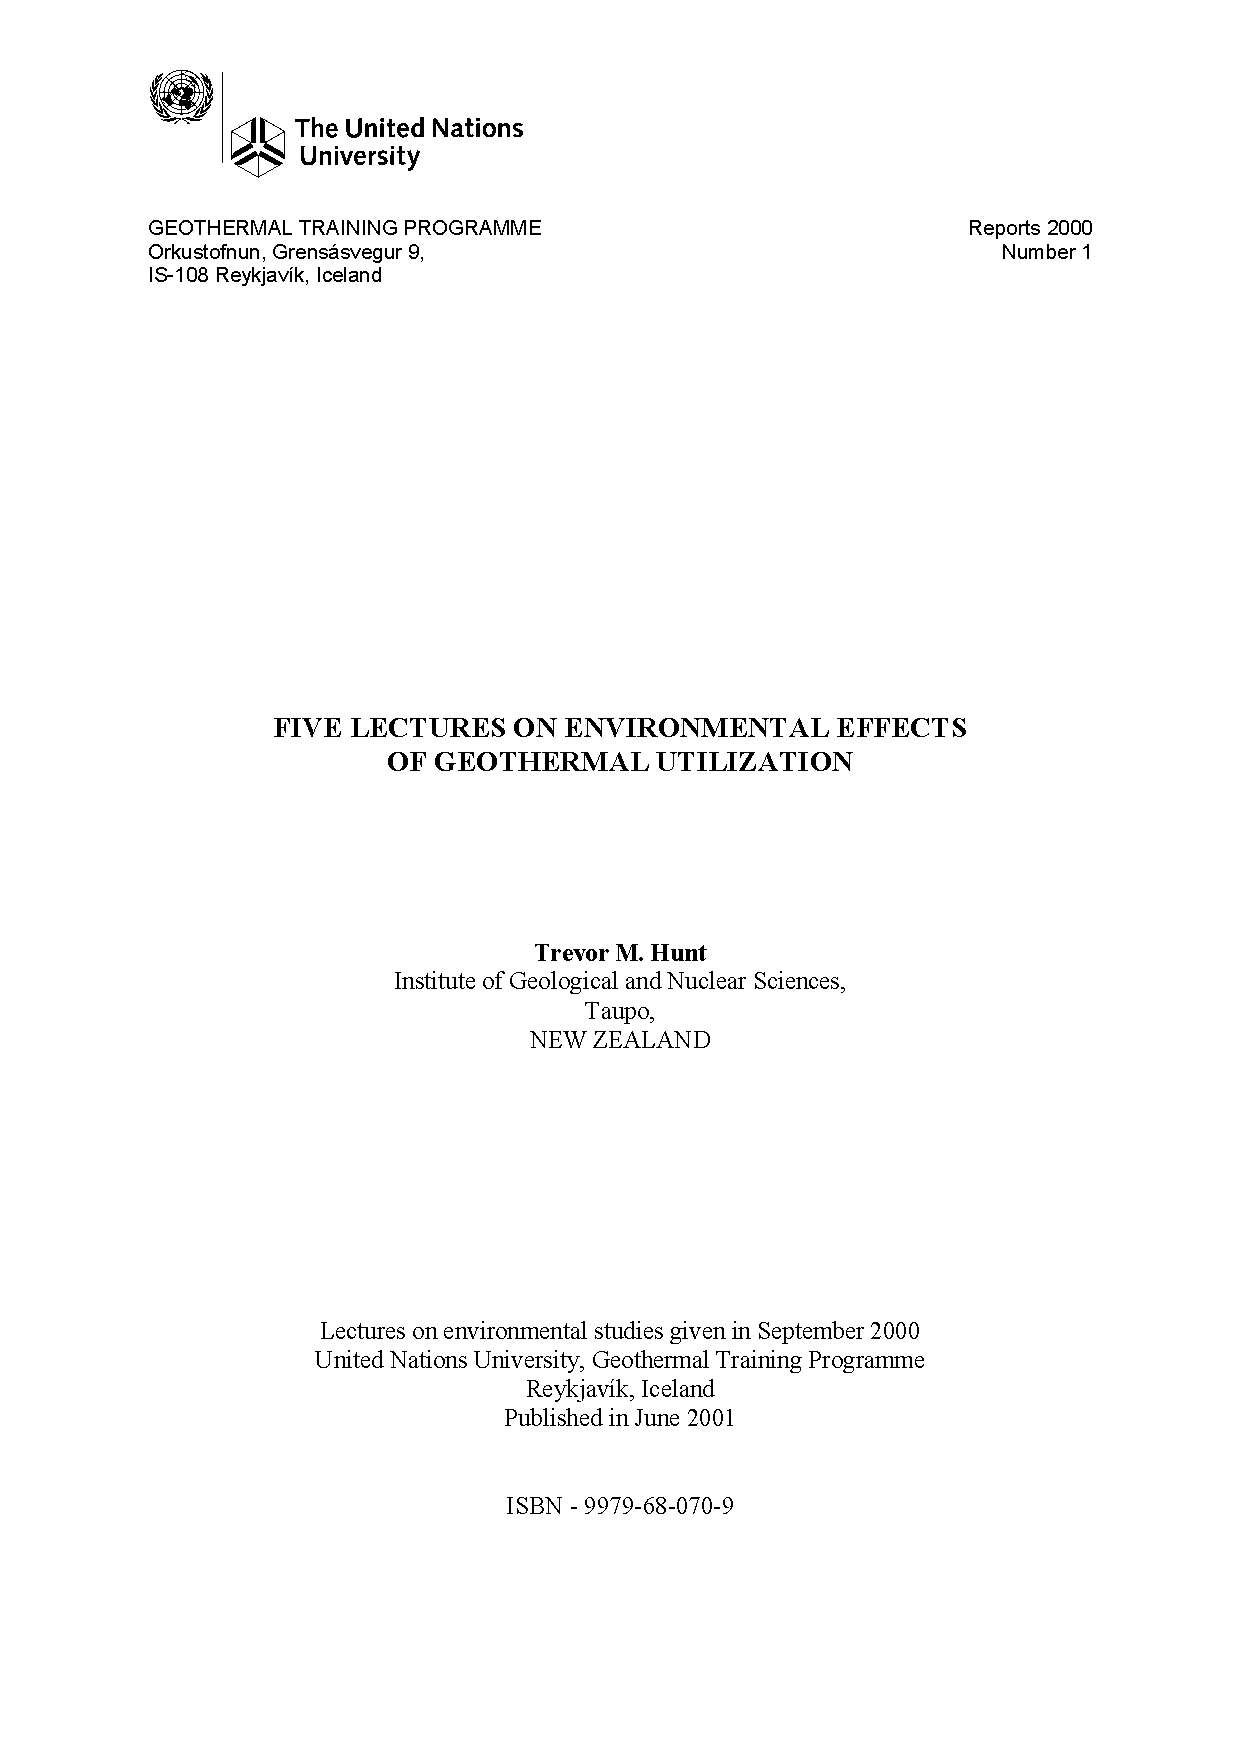
\includepdf[pages=-,fitpaper, angle=0]{./HuntSelect.pdf}
%}

\end{document}
